% TAIMMA 2027 submission, Springer LNCS format (llncs v2.25, splncs04).
% Full papers: 12-15 pages including references.
% Double-blind review format configured for submission.
\documentclass[runningheads]{llncs}

\usepackage[T1]{fontenc}
\usepackage{amsmath,amssymb}
\IfFileExists{newtxtext.sty}{%
  \usepackage{newtxtext}
  \usepackage[varvw]{newtxmath}
}{%
  \usepackage{mathptmx}
}
\usepackage{graphicx}
\usepackage{booktabs}
\usepackage{tabularx}
\usepackage{multirow}
\usepackage{microtype}
\usepackage{color}
\usepackage{hyperref}
\hypersetup{
  colorlinks=true,
  linkcolor=blue,
  citecolor=blue,
  urlcolor=blue,
  bookmarksnumbered=true,
  bookmarksopen=true
}
\setcounter{tocdepth}{2}
\renewcommand\UrlFont{\color{blue}\rmfamily}
\urlstyle{rm}

\begin{document}

\title{Why a Cheaper Block Runs Slower: Replacing Self-Attention with 2D Selective Scans in YOLO11s on an Embedded CPU}
\titlerunning{Why a Cheaper Block Runs Slower}

% Single-blind review: authors and institute included per TAIMMA 2027 policy
\author{Vo Tuan Hung\inst{1}\orcidID{0009-0005-8730-7930} \and
Huynh Tan Phat\inst{2}\thanks{Corresponding author.}}
\authorrunning{T. H. Vo and T. P. Huynh}
\institute{Information Technology Department, Song Hung Thuan Co., Ltd.,\\
50C Hanoi Highway, Phuoc Long Ward, Ho Chi Minh City, Vietnam\\
\email{votuanhung1205.work@gmail.com}
\and
Ho Chi Minh City Open University, Ho Chi Minh City, Vietnam\\
\email{phat.ht@ou.edu.vn}}

\maketitle

\begin{abstract}
Selective state space models (SSMs) offer global context at linear cost, but their cost inside lightweight detectors on embedded CPUs is poorly characterized. We replace the $P_5$ self-attention block (\texttt{C2PSA}) of YOLO11s with a plugin-free, four-direction 2D selective scan (SS2D), and study its accuracy on a cross-facility partition of the synthetic NVIDIA PhysicalAI-SmartSpaces warehouse benchmark and its deployment cost on a Raspberry Pi~4. The replacement removes $6.72\%$ of the parameters and about $0.44$ GFLOPs, mainly by narrowing channels. In preliminary single-seed experiments with single-stage, two-stage, and dual-scale training, we do not observe accuracy preservation: the baseline leads at the final epoch in $\text{mAP}_{50}$ and $\text{mAP}_{50-95}$, although one seed cannot separate this from run-to-run variance. We call a model edge-feasible if it runs in FP32 ONNX Runtime without custom operators within $1$\,GiB of peak memory; the SS2D model meets this criterion but is $18\%$ slower than the baseline with four threads ($1314$ vs.\ $1117$\,ms forward latency) and uses $60\%$ more peak memory despite fewer FLOPs. Profiling and runtime interventions show that the overhead comes from how the scan is executed rather than its arithmetic or graph size: re-expressing the same scan as an ONNX \texttt{Loop} with $40\times$ fewer nodes, as a chunked scan, or as a parallel associative scan without the sequential chain made the model slower, and removing $68\%$ of the scan core's multiply-accumulates did not lower latency. We summarize design lessons for hybrid CNN--SSM detectors on edge CPUs, including a pitfall in zero-initializing a convolution ahead of batch normalization.

\keywords{Object detection \and YOLO \and Mamba \and State space models \and Edge AI \and Warehouse perception.}
\end{abstract}

\section{Introduction}
\label{sec:introduction}
Automated warehouses mix workers, forklifts, pallet trucks, and autonomous mobile robots (AMRs) in shared aisles, so multi-class object detection is a basic requirement for their safe operation. Detectors in this setting face large scale and viewpoint variation, repetitive racking with frequent occlusion, and the compute, memory, and thermal limits of single-board computers such as the Raspberry Pi~4.

Lightweight convolutional detectors such as YOLO11s~\cite{ultralytics2024yolo11} run efficiently on such devices, but each convolution aggregates only local context. YOLO11s therefore adds one self-attention block, \texttt{C2PSA}, at its lowest-resolution stage $P_5$; it holds $990{,}976$ parameters (about $10.5\%$ of the model), although at the $20 \times 20$ resolution of $P_5$ ($N = 400$ tokens) its quadratic cost $\mathcal{O}(N^2)$ is small in absolute terms. Selective state space models (SSMs) such as Mamba~\cite{gu2023mamba} and their visual variants~\cite{liu2024vmamba,zhu2024visionmamba} offer global context with cost linear in $N$, and several works have inserted them into YOLO-style detectors~\cite{wang2025mambayolo,lei2025mambanext,chan2026mambapsa}. These works report accuracy, FLOPs, or GPU and Jetson throughput; the measured cost of a plugin-free scan on an embedded CPU, and what determines it, has received little attention.

We therefore ask three research questions. \textbf{RQ1:} Does replacing the $P_5$ attention block of YOLO11s with a simplified, plugin-free 2D selective-scan block preserve accuracy while reducing parameters and FLOPs? \textbf{RQ2:} Does inserting a newly initialized scan block into a pretrained detector require a dedicated protocol (two-stage training, identity initialization)? \textbf{RQ3:} What latency and memory does a plugin-free selective scan incur on an embedded CPU, and which implementation factors determine that cost?

This is primarily a systems and measurement study of deployment cost; the block itself is a simplified variant of existing designs. Our contributions are as follows:
\begin{itemize}
    \item \textbf{A hardware-counter autopsy of embedded SSM cost} on a Raspberry Pi~4 (ARM Cortex-A72). Despite reducing theoretical complexity ($-6.72\%$ parameters, $-0.44$ GFLOPs), the SS2D detector is $18\%$ slower than the attention baseline ($1314$ vs.\ $1117$\,ms with four threads) and uses $60\%$ more peak memory ($373.6$ vs.\ $233.4$\,MiB). Using controlled graph interventions and hardware counters (\texttt{perf stat}), we prove that this penalty does not stem from arithmetic FLOPs, but from operator dispatch overhead in the unrolled sequential scan ($14{,}771$ nodes) and severe memory-bandwidth pressure in the parallel scan ($2.2\times$ DRAM traffic, $2.5\times$ L2 refills).
    \item \textbf{A fine-grained per-component cost breakdown of replacing \texttt{C2PSA}} with a plugin-free 4-direction selective scan. We reveal that the $63.9\%$ Layer-10 parameter saving stems from narrower channel projections rather than the token-mixing core, and that redundant per-direction parameter projection makes the core more expensive than self-attention at $L = 400$.
    \item \textbf{An analysis of CNN--SSM grafting pitfalls.} We show that zero-initializing a projection convolution ahead of batch normalization preserves identity only at step 0, explaining the early-epoch gradient instability that necessitated two-stage warmup, and show that the trained scan acts primarily as a localized mixer.
\end{itemize}

\section{Related Work}
\label{sec:related_work}

\subsection{YOLO Detectors and Visual State Space Models}
Since the single-stage formulation of YOLO~\cite{redmon2016yolo}, the family has moved to anchor-free heads and, in YOLO11, to \texttt{C3k2} blocks and the \texttt{C2PSA} block, which wraps the partial self-attention module introduced in YOLOv10~\cite{wang2024yolov10}; YOLO26 adds NMS-free inference~\cite{sapkota2026ultralytics}. Apart from \texttt{C2PSA}, small YOLO11 models rely entirely on local convolutions. Selective SSMs such as Mamba~\cite{gu2023mamba} use input-dependent state transitions with cost linear in sequence length, and visual variants such as Vision Mamba~\cite{zhu2024visionmamba} and VMamba~\cite{liu2024vmamba} flatten 2D feature maps along several scan directions (the four-way cross-scan, SS2D, of VMamba). The linear scaling matters most at high resolution; at the deepest stage of a detector its benefit is an empirical question.

\subsection{Hybrid CNN--Mamba Detectors}
Table~\ref{tab:lit_comparison} lists the hybrid detectors closest to this work. Mamba YOLO~\cite{wang2025mambayolo} builds an SSM-based backbone (ODMamba) with a multi-branch RG Block and reports GPU inference on COCO. MambaNeXt-YOLO~\cite{lei2025mambanext} combines convolutions and Mamba in a MambaNeXt block, evaluates on PASCAL VOC, and reports deployment on Jetson Xavier NX and Orin NX devices. Closest to our work, MambaPSA~\cite{chan2026mambapsa} replaces \texttt{C2PSA} in YOLO26 with a Mamba-based block and reports PASCAL VOC accuracy and CPU throughput. Xray-YOLO-Mamba~\cite{zhao2025xraymamba} applies selective SSMs to X-ray images. Our study differs in domain (cross-facility warehouse detection), in hardware (an embedded ARM CPU), and in its operator-level analysis of deployment cost; it does not propose a fundamentally different block. MambaOut~\cite{yu2024mambaout} argues that SSMs are unnecessary for ImageNet classification but may remain useful for dense tasks, which motivates convolution-only controls; we include such controls as untrained runtime references only (Section~\ref{sec:res_edge}).

\begin{table}[t]
\caption{Hybrid CNN--Mamba detectors closest to this work, as described by their authors.}
\label{tab:lit_comparison}
\centering
\footnotesize
\setlength{\tabcolsep}{3pt}
\begin{tabularx}{\textwidth}{>{\raggedright\arraybackslash}p{2.3cm} >{\raggedright\arraybackslash}p{2.1cm} >{\raggedright\arraybackslash}X >{\raggedright\arraybackslash}p{2.9cm}}
\toprule
\textbf{Model} & \textbf{Evaluation data} & \textbf{SSM placement} & \textbf{Reported deployment} \\
\midrule
Mamba YOLO~\cite{wang2025mambayolo} & MS COCO & ODMamba backbone with RG Blocks & Desktop GPU (RTX 4090) \\
MambaNeXt-YOLO~\cite{lei2025mambanext} & PASCAL VOC & MambaNeXt blocks; fusion pyramid & Jetson Xavier NX, Orin NX \\
MambaPSA~\cite{chan2026mambapsa} & PASCAL VOC & Replaces \texttt{C2PSA} in YOLO26 & CPU (17 to 20 FPS) \\
\midrule
This work & Synthetic warehouse, cross-facility & $P_5$ (and $P_4$), replaces \texttt{C2PSA} in YOLO11s & Raspberry Pi~4 CPU, ONNX Runtime \\
\bottomrule
\end{tabularx}
\end{table}

\subsection{Edge Deployment and Warehouse Perception}
Parameter counts and FLOPs are poor predictors of on-device latency: memory access cost and the fragmentation of a model into many small, non-fused operators often dominate runtime~\cite{ma2018shufflenetv2,mittal2024lightweightsurvey}, and runtimes such as ONNX Runtime and TensorRT gain much of their speed from operator fusion~\cite{ratul2024accelerating}. In warehouses, Yang et~al.~\cite{yang2024freezerwarehouse} designed a lightweight detector for food freezer warehouses, and the NVIDIA PhysicalAI-SmartSpaces benchmark~\cite{wang2026smartspaces} provides multi-camera data from many synthetic facilities, which enables cross-facility evaluation. We are not aware of prior work that evaluates a selective-scan replacement for the YOLO attention block on multi-class warehouse detection with measurements on a single-board ARM computer.

\section{Method}
\label{sec:methodology}

\subsection{Architecture}
\label{sec:arch_overview}
The detector predicts boxes for four classes: \texttt{worker}, \texttt{forklift}, \texttt{pallet\_truck}, and \texttt{amr}. It keeps the YOLO11s backbone (Layers 0--9, ending with \texttt{SPPF}), its FPN/PAN neck, and its decoupled anchor-free \texttt{Detect} head, trained with the Ultralytics CIoU, binary cross-entropy, and distribution focal losses. In \textbf{SS2D-P5}, the \texttt{C2PSA} block at Layer~10 is replaced by a shape-compatible \texttt{WarehouseSS2DBlock}, $[b, 512, 20, 20] \to [b, 512, 20, 20]$, at stage $P_5$. \textbf{SS2D-P4P5} adds a second block at $P_4$ ($[b, 256, 40, 40]$, Layer~7). Fig.~\ref{fig:arch_diagram} shows the block.

\begin{figure}[t]
\centering
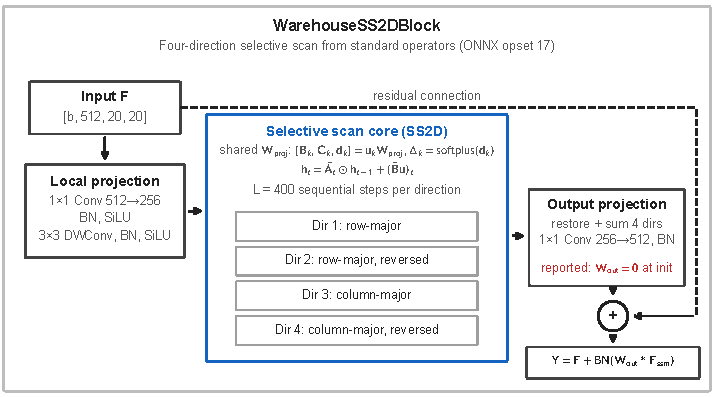
\includegraphics[width=\textwidth]{figures/fig_ss2d_block.pdf}
\caption{The \texttt{WarehouseSS2DBlock} that replaces \texttt{C2PSA} at Layer~10. The red label marks the $\mathbf{W}_{\text{out}} = \mathbf{0}$ initialization used for all reported models (Eq.~\eqref{eq:zero_wout}).}
\label{fig:arch_diagram}
\end{figure}

\subsection{Warehouse SS2D Block}
\label{sec:mamba_integration}
A $1 \times 1$ convolution projects the $C_{\text{in}} = 512$ input channels of $\mathbf{F}$ to $d_{\text{inner}} = 256$ channels and a depthwise $3 \times 3$ convolution adds local context, each followed by batch normalization (BN) and SiLU, giving $\mathbf{F}_{\text{dw}} \in \mathbb{R}^{b \times d_{\text{inner}} \times H \times W}$. $\mathbf{F}_{\text{dw}}$ is flattened along four traversal orders of the $L = H \times W = 400$ grid: row-major, reversed row-major, column-major, and reversed column-major, giving sequences $\mathbf{u}_k \in \mathbb{R}^{b \times L \times d_{\text{inner}}}$, $k = 1, \dots, 4$. A projection $\mathbf{W}_{\text{proj}} \in \mathbb{R}^{d_{\text{inner}} \times (2 d_{\text{state}} + d_{\text{inner}})}$, shared by all directions, produces the input-dependent parameters
\begin{equation}
    [\mathbf{B}_k, \mathbf{C}_k, \mathbf{d}_k] = \mathbf{u}_k \mathbf{W}_{\text{proj}}, \quad \boldsymbol{\Delta}_k = \operatorname{softplus}(\mathbf{d}_k),
\end{equation}
which are discretized as $\overline{\mathbf{A}}_k = \exp(\boldsymbol{\Delta}_k \odot \mathbf{A}_k)$, the exact zero-order hold for the diagonal state matrix $\mathbf{A}_k = -\exp(\mathbf{A}_{\text{log}, k})$, and $(\overline{\mathbf{B}}\mathbf{u})_k = (\boldsymbol{\Delta}_k \odot \mathbf{u}_k) \odot \mathbf{B}_k$, a first-order approximation of the input term ($\odot$ broadcasts element-wise). With $d_{\text{state}} = 16$, the hidden state $\mathbf{h}_{k,t} \in \mathbb{R}^{d_{\text{inner}} \times d_{\text{state}}}$ is updated over $t = 1, \dots, L$:
\begin{equation}
    \mathbf{h}_{k,t} = \overline{\mathbf{A}}_{k,t} \odot \mathbf{h}_{k,t-1} + (\overline{\mathbf{B}}\mathbf{u})_{k,t}, \qquad
    \mathbf{y}_{k,t} = \textstyle\sum_{n=1}^{d_{\text{state}}} \mathbf{h}_{k,t,n} \odot \mathbf{C}_{k,t,n} + \mathbf{D}_k \odot \mathbf{u}_{k,t}.
\end{equation}
The four outputs are restored to row-major order and summed into $\mathbf{F}_{\text{ssm}}$, which a $1 \times 1$ convolution $\mathbf{W}_{\text{out}}$ and BN map back to $512$ channels before the residual sum $\mathbf{Y} = \mathbf{F} + \operatorname{BN}_{\gamma, \beta}(\mathbf{W}_{\text{out}} * \mathbf{F}_{\text{ssm}})$.

Compared with Mamba~\cite{gu2023mamba} and VMamba~\cite{liu2024vmamba}, the block has no multiplicative gating branch, uses a full-rank step-size projection without bias or Mamba's step-size initialization, initializes $\mathbf{A}_{\text{log}}$ from a standard normal distribution rather than S4D-real, and shares $\mathbf{W}_{\text{proj}}$ across directions. These simplifications keep the block small and export-friendly but have not been ablated, so our results should not be read as representative of a standard Mamba block. They also shorten the effective memory of the scan: on $10$ validation frames, the trained $P_5$ scans of Arms~2 and~3 have a median per-step decay $\overline{\mathbf{A}}$ of $0.52$, so a state entry falls to $1/e$ within a median of $1.5$ tokens ($99$th percentile $16$), and only $0.5\%$ of entries persist over one $20$-token row. The block lacks Mamba's small step-size initialization, and after training the decay per step remains fast, so the scan mixes information mostly locally along each direction.

\textbf{Initialization.} To avoid perturbing pretrained features, all reported models zero-initialize the output convolution and keep the default BN parameters:
\begin{equation}
    \mathbf{W}_{\text{out},0} = \mathbf{0}, \; \gamma_0 = \mathbf{1}, \; \beta_0 = \mathbf{0} \implies \mathbf{Y}_0 \equiv \mathbf{F}.
    \label{eq:zero_wout}
\end{equation}
Eq.~\eqref{eq:zero_wout} is thus a valid but weaker identity initialization, exact only at step $0$: once $\mathbf{W}_{\text{out}}$ becomes small but nonzero, BN rescales its output to unit variance, so with $\gamma = \mathbf{1}$ the untrained branch contributes at full scale from the first iterations. We hypothesize, without having tested it, that this contributes to the unstable early-epoch validation metrics that motivated two-stage training. Following the zero-$\gamma$ residual principle~\cite{goyal2017accurate}, our current implementation instead sets
\begin{equation}
    \gamma_0 = \mathbf{0}, \; \beta_0 = \mathbf{0} \implies \mathbf{Y}_0 \equiv \mathbf{F},
    \label{eq:zero_gamma}
\end{equation}
so that the branch grows gradually with $\gamma$ while $\partial \mathbf{Y} / \partial \gamma = \hat{\mathbf{Z}} \neq \mathbf{0}$ keeps it trainable. We verified this on an isolated block but have not retrained the detectors with it: all reported models use Eq.~\eqref{eq:zero_wout}, and the effect of Eq.~\eqref{eq:zero_gamma} on accuracy is untested.

\subsection{Analytical Cost}
\label{sec:complexity}
The replacement reduces Layer~10 from $990{,}976$ to $357{,}632$ parameters ($-63.9\%$) and the model from $9{,}429{,}340$ to $8{,}795{,}996$ parameters ($-6.72\%$) and from $21.7$ to $21.2$ GFLOPs at $640 \times 640$. Table~\ref{tab:layer10_breakdown} shows where the savings come from. The token-mixing cores are both small: the attention products of \texttt{C2PSA} ($h L^2 (d_k + d_v)$ with $h = 4$, $d_k = 32$, $d_v = 64$) cost $61.4$\,M MACs, and the SS2D parameter projection ($K L d (2s + d)$ with $K = 4$, $d = 256$, $s = 16$) and recurrence ($\approx 2 K L d s$) cost $118.0$ and $13.1$\,M MACs, each at most about $1\%$ of the roughly $10.8$ GMACs of the model. As implemented, the core is thus not cheaper than attention. The projection is, however, applied to each of the $K = 4$ permuted sequences; because it acts per token and the directions are permutations of the same tokens, projecting once and permuting the result is identical (maximum difference $3 \times 10^{-15}$ in float64) and would cost $29.5$\,M MACs, making the core ($42.6$\,M) cheaper than attention. All accuracy results use the per-direction projection; Section~\ref{sec:res_edge} measures the once-projected export. The net saving of $633{,}344$ parameters and about $219$\,M MACs ($\approx 0.44$ GFLOPs) comes from narrower $512 \leftrightarrow 256$ projections and the removal of the feed-forward network. The decisive difference is the sequential dependency chain: attention has none across tokens, whereas the reference scan runs $K = 4$ independent chains of $L = 400$ dependent steps.

\begin{table}[t]
\caption{Per-component cost of Layer~10 at $P_5$ ($20 \times 20$). BN: batch-normalization affine parameters. --: no learnable weights, or negligible cost.}
\label{tab:layer10_breakdown}
\centering
\footnotesize
\setlength{\tabcolsep}{4pt}
\begin{tabular}{llrr}
\toprule
\textbf{Block} & \textbf{Component} & \textbf{Params} & \textbf{MACs (M)} \\
\midrule
\multirow{8}{*}{\texttt{C2PSA}} & \texttt{cv1} $1\times1$, $512 \to 512$ & 262,144 & 104.9 \\
 & \texttt{qkv} $1\times1$, $256 \to 512$ & 131,072 & 52.4 \\
 & \texttt{proj} $1\times1$, $256 \to 256$ & 65,536 & 26.2 \\
 & Positional DWConv $3\times3$ & 2,304 & 0.9 \\
 & Attention $QK^{\top}$, $AV$ & -- & 61.4 \\
 & FFN $256 \to 512 \to 256$ & 262,144 & 104.9 \\
 & \texttt{cv2} $1\times1$, $512 \to 512$ & 262,144 & 104.9 \\
 & BN & 5,632 & -- \\
\cmidrule(lr){2-4}
 & \textbf{Total} & \textbf{990,976} & \textbf{455.6} \\
\midrule
\multirow{7}{*}{SS2D} & In-projection $1\times1$, $512 \to 256$ & 131,072 & 52.4 \\
 & DWConv $3\times3$ & 2,304 & 0.9 \\
 & $\mathbf{W}_{\text{proj}}$ (applied per direction; once: $29.5$) & 73,728 & 118.0 \\
 & $\mathbf{A}_{\text{log}}$, $\mathbf{D}$ & 17,408 & -- \\
 & Recurrence and readout ($4 \times 400$ sequential steps) & -- & 13.1 \\
 & Out-projection $1\times1$, $256 \to 512$ & 131,072 & 52.4 \\
 & BN & 2,048 & -- \\
\cmidrule(lr){2-4}
 & \textbf{Total} & \textbf{357,632} & \textbf{236.8} \\
\bottomrule
\end{tabular}
\end{table}

\subsection{Two-Stage Training}
\label{sec:training_workflow}
Because early trials showed unstable early-epoch validation metrics after inserting a new block, we also evaluate a two-stage protocol: in stage~1, Layers 0--9 are frozen (\texttt{freeze=10}) for $5$ epochs, so only the SS2D block, neck, and head are updated (BN running statistics in frozen layers still update); in stage~2, all parameters are trained for $15$ epochs from the stage-1 weights. Each stage is a separate Ultralytics run, so stage~2 restarts the learning-rate warmup and decay.

\section{Experimental Setup}
\label{sec:experimental_setup}

\subsection{Data}
\label{sec:exp_datasets}
We use the warehouse scenes of the NVIDIA PhysicalAI-SmartSpaces benchmark (MTMC tracking data)~\cite{wang2026smartspaces}, rendered with NVIDIA Omniverse, and partition them by facility. Training uses two cameras of \texttt{Warehouse\_000} sampled at $0.5$\,FPS ($300$ frames, $12{,}959$ boxes); validation uses two cameras of the different facility \texttt{Warehouse\_015} ($100$ frames, $3{,}696$ boxes). Sampling at $0.5$\,FPS reduces the redundancy between consecutive frames and keeps CPU training tractable; with static cameras, frames $2$\,s apart remain strongly correlated (Section~\ref{sec:limitations}). No facility, camera, or video sequence is shared, but 3D assets such as forklift and robot models come from the same library, so object appearance is not independent across partitions, and all views are static simulated cameras. The training/validation instances are \texttt{worker} $11{,}399$/$3{,}488$, \texttt{forklift} $600$/$150$, \texttt{amr} $724$/$45$, and \texttt{pallet\_truck} $236$/$13$; the validation partition is therefore strongly imbalanced ($94.37\%$ workers, $0.35\%$ pallet trucks). Boxes with a side of at most $4$ pixels are removed and frames are letterboxed from $1920 \times 1080$ to $640 \times 640$. All arms use the Ultralytics default augmentation, in which mosaic is switched off for the last $10$ epochs (\texttt{close\_mosaic=10}).

\subsection{Experimental Arms and Training}
\label{sec:exp_baselines}
\textbf{Arm~1} is the unmodified YOLO11s ($9.43$\,M parameters, $21.7$ GFLOPs). \textbf{Arm~2} trains SS2D-P5 ($8.80$\,M, $21.2$ GFLOPs) in a single stage, \textbf{Arm~3} trains SS2D-P5 with the two-stage protocol, and \textbf{Arm~4} trains SS2D-P4P5 ($8.89$\,M, $21.8$ GFLOPs) in a single stage. All arms are fine-tuned from the same COCO checkpoint for $20$ epochs; only the SS2D blocks start untrained. The comparison is not a single-variable intervention: \texttt{C2PSA} starts pretrained whereas the SS2D blocks receive only about $1{,}500$ optimizer steps, and Arm~3 differs from Arm~2 both in freezing and in its restarted schedule.

Training used Python 3.14.8, PyTorch 2.14.1, and Ultralytics (8.4.185 for Arms 1--3 and 8.4.187 for Arm~4, read from the checkpoints), with AdamW selected by \texttt{optimizer=auto} ($\eta = 0.00125$, $\beta_1 = 0.9$, linear decay to $0.01\eta$ after a $3$-epoch warmup, weight decay $0.0005$), batch size $4$, input size $640$, and seed $0$ (one run per arm) on a host CPU workstation. We report the final-epoch model and the checkpoint with the highest validation fitness ($0.1\,\text{mAP}_{50} + 0.9\,\text{mAP}_{50-95}$); because both are evaluated on the partition used for selection, best-fitness figures are optimistically biased. Metrics are class-macro $\text{mAP}_{50}$ and $\text{mAP}_{50-95}$, and precision and recall at the confidence threshold that maximizes F1.

\subsection{Edge Measurement Protocol}
\label{sec:exp_export}
Checkpoints are exported to ONNX (opset 17, \texttt{onnxslim}) with standard operators only. The Pi files are the exports of the trained best checkpoints of Arm~1 (baseline), Arm~3 (SS2D-P5), and Arm~4 (SS2D-P4P5), identified by SHA-256 hashes; an earlier SS2D-P5 measurement that mistakenly used a pre-fine-tuning export is superseded. Models run in ONNX Runtime 1.31 (CPU execution provider, FP32, \texttt{ORT\_ENABLE\_ALL}, batch size $1$) on an Intel Core i7-7600U host (default threads) and on a Raspberry Pi~4 Model~B Rev~1.2 (Cortex-A72, $1.5$\,GHz, 4\,GB; Debian 13, Python 3.13.5; no heatsink or fan; official 5\,V/3\,A power supply) with $1$ or $4$ intra-op threads. We call a model \emph{edge-feasible} on the Pi if it runs there in FP32 without custom operators or plugins and within $1$\,GiB of peak memory; this criterion does not imply real-time throughput.

\textbf{Latency} is the time of \texttt{session.run} on a fixed input after untimed warmup, without preprocessing or NMS; we report the median, mean $\pm$ SD, and FPS $= 1000/\text{median}$. Single-thread runs use $10$ warmup and $100$ timed calls; four-thread runs use $5$ warmup and $30$ timed calls, because $100$-call runs heated the SoC to $79$--$84\,^{\circ}$C and once lowered the clock to $1.23$--$1.48$\,GHz; those runs are discarded. Every reported run started below $55\,^{\circ}$C. The Pi results come from three sessions: session~1 (baseline and SS2D-P4P5; clock logged only for the four-thread runs, which stayed at $1.5$\,GHz), session~2 (baseline, SS2D-P5, and the untrained intervention below; clock logged throughout, $1.5$\,GHz whenever a model ran, at most $76.9\,^{\circ}$C), and session~3 (the parallel scan below with its controls; clock logged throughout, at most $75.9\,^{\circ}$C). Relative values use the baseline of the same session. \textbf{Memory} is the peak resident set size of the process (\texttt{VmHWM}, including Python and session creation) on the Pi, and the RSS after the timed loop on the host. \textbf{Operator profiles} use the ONNX Runtime profiler with four threads and $5$ profiled calls after $2$ warmup calls.

\textbf{Runtime intervention.} To test whether graph size drives latency, we export the same SS2D block in three graph forms: the unrolled sequential scan used above, the same recurrence as one ONNX \texttt{Loop} per direction, and a chunked scan with chunk size $T = 4$. As runtime references we also export the baseline, the model with the $P_5$ block removed (identity), and a convolution-only replacement. These exports use untrained weights (seed $0$, BN statistics calibrated on random inputs, $\gamma = 1$), because they are compared only with each other. The three SS2D forms produce the same outputs (maximum relative difference $2.3 \times 10^{-6}$, versus $0.154$ between the SS2D and convolution-only exports as a negative control). Each runs with $1$ and $4$ threads, $3$ warmup and $20$ timed calls, in session~2. To test whether the sequential dependency chain drives latency, we also export the trained Arm~3 weights with the scan evaluated as a parallel (Hillis--Steele) associative scan~\cite{blelloch1990prefix}, which combines each position with the one $k = 1, 2, 4, \dots$ steps earlier and thus needs $\lceil \log_2 L \rceil$ steps instead of $L$; it matches the sequential recurrence to $2.8 \times 10^{-14}$ in float64 and the measured Arm~3 export to a relative output difference of $1.9 \times 10^{-7}$. It runs in session~3 with the trained baseline and unrolled Arm~3 exports as controls, under the protocol of the main measurements.

\section{Results and Discussion}
\label{sec:results}

\subsection{Detection Accuracy}
\label{sec:res_detection}
Table~\ref{tab:accuracy_results} summarizes accuracy after identical 20-epoch budgets, and Fig.~\ref{fig:convergence_map} shows the validation curves. Two views must be distinguished. At the \emph{final epoch}, the baseline leads with $69.75\%\ \text{mAP}_{50}$, ahead of Arm~4 ($67.17\%$), Arm~3 ($67.10\%$), and Arm~2 ($65.46\%$), and with $45.83\%\ \text{mAP}_{50-95}$ versus $41.56$--$43.17\%$. At the \emph{best-fitness checkpoint}, Arm~2 reaches $71.95\%$ (epoch 18) versus $69.80\%$ for the baseline (epoch 20), but this checkpoint is selected on the same $100$ frames on which it is reported, so the figure is optimistically biased and we do not interpret it as evidence for SS2D. All SS2D arms have lower $\text{mAP}_{50-95}$ under either view. Validation $\text{mAP}_{50}$ also changes by up to $14$ points between consecutive epochs after epoch $5$, and by up to $33$ points in the first epochs of Arm~4, which exceeds the $+2.15$-point gap between Arm~2 and the baseline; switching off mosaic at epoch $11$ may contribute. With a single seed, differences between arms cannot be distinguished from run-to-run variance.

\begin{table}[t]
\caption{Accuracy on the validation partition (single seed). Best-fitness checkpoints are selected on the same partition and are therefore optimistically biased; P and R refer to them, the box loss to the final epoch. Arm~3 epochs are counted within stage~2. Final-epoch values come from the validation run during training, best-fitness values from a standalone re-validation of \texttt{best.pt}; for Arms~1 and~4, whose best checkpoint is the final epoch, the two differ by at most $0.3$ points.}
\label{tab:accuracy_results}
\centering
\footnotesize
\setlength{\tabcolsep}{2.6pt}
\begin{tabular}{lccccccc}
\toprule
 & \multicolumn{2}{c}{\textbf{Final epoch}} & \multicolumn{2}{c}{\textbf{Best fitness}} & & & \textbf{Final val.} \\
\cmidrule(lr){2-3} \cmidrule(lr){4-5}
\textbf{Arm} & $\textbf{mAP}_{50}$ & $\textbf{mAP}_{50-95}$ & $\textbf{mAP}_{50}$ (ep.) & $\textbf{mAP}_{50-95}$ & \textbf{P} & \textbf{R} & \textbf{box loss} \\
\midrule
1: Baseline & \textbf{69.75} & \textbf{45.83} & 69.80 (20) & \textbf{45.53} & \textbf{0.818} & 0.572 & \textbf{1.0196} \\
2: SS2D, single-stage & 65.46 & 41.56 & \textbf{71.95} (18) & 45.15 & 0.744 & 0.576 & 1.0688 \\
3: SS2D, two-stage & 67.10 & 43.17 & 67.67 (14) & 43.15 & 0.741 & \textbf{0.651} & 1.0512 \\
4: SS2D, dual-scale & 67.17 & 42.73 & 67.17 (20) & 42.76 & 0.738 & 0.515 & 1.0863 \\
\bottomrule
\end{tabular}
\end{table}

\begin{figure}[t]
\centering
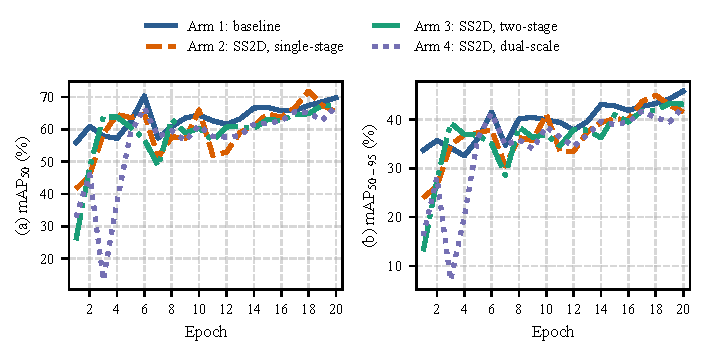
\includegraphics[width=\textwidth]{figures/fig_convergence_map_wide.pdf}
\caption{Validation (a) $\text{mAP}_{50}$ and (b) $\text{mAP}_{50-95}$ over 20 epochs (one seed per arm, so no run-to-run variance is shown). For Arm~3, epochs 1--5 are stage~1 and epochs 6--20 are stage-2 epochs 1--15, so its best-fitness checkpoint (stage-2 epoch 14) appears at epoch 19.}
\label{fig:convergence_map}
\end{figure}

Two-stage training (Arm~3) has the highest recall ($0.651$ vs.\ $0.572$ for the baseline) but lower precision ($0.741$ vs.\ $0.818$). Because both are reported at the F1-maximizing threshold, this is mainly a shift of the operating point: the derived F1 is $0.693$ vs.\ $0.673$, and $0.683$ vs.\ $0.673$ at the final epoch. The dual-scale model (Arm~4) is close to Arm~3, so adding a $P_4$ block brings no measurable benefit here at a substantial runtime cost. In an initial version of the SS2D pipeline, adapting the COCO head to four classes also re-initialized the $42$ class-agnostic box-regression tensors, raising the initial box loss to $6.276$; transferring all shape-compatible tensors, as Ultralytics does for the baseline, lowers it to $2.758$, and all reported SS2D models use this correction.

\begin{table}[t]
\caption{Per-class $\text{mAP}_{50}$ / $\text{mAP}_{50-95}$ (\%) of the best-fitness checkpoints on the validation partition (also used for checkpoint selection).}
\label{tab:per_class_results}
\centering
\footnotesize
\setlength{\tabcolsep}{4pt}
\begin{tabular}{lcccc}
\toprule
\textbf{Class (val.\ instances)} & \textbf{Arm 1} & \textbf{Arm 2} & \textbf{Arm 3} & \textbf{Arm 4} \\
\midrule
\texttt{worker} ($3{,}488$) & 89.2 / \textbf{63.2} & \textbf{89.4} / 61.9 & 87.9 / 60.5 & 88.5 / 60.9 \\
\texttt{forklift} ($150$) & 70.1 / 31.8 & \textbf{79.7} / 38.3 & 76.3 / \textbf{38.4} & 75.3 / 33.8 \\
\texttt{pallet\_truck}$^{\dagger}$ ($13$) & 32.8 / \textbf{22.4} & \textbf{33.9} / 17.7 & 22.9 / 16.2 & 20.0 / 14.6 \\
\texttt{amr} ($45$) & \textbf{87.1} / \textbf{64.7} & 84.9 / 62.6 & 83.7 / 57.5 & 85.0 / 61.7 \\
\midrule
Macro (4 classes) & 69.80 / \textbf{45.53} & \textbf{71.95} / 45.15 & 67.67 / 43.15 & 67.17 / 42.76 \\
Macro (3 classes)$^{\ddagger}$ & 82.1 / 53.2 & \textbf{84.7} / \textbf{54.3} & 82.6 / 52.1 & 82.9 / 52.1 \\
\bottomrule
\multicolumn{5}{p{0.92\textwidth}}{\scriptsize $^{\dagger}$Only $13$ validation instances ($0.35\%$ of labels); not interpreted. $^{\ddagger}$Without \texttt{pallet\_truck}, from the rounded per-class values.} \\
\end{tabular}
\end{table}

Per class (Table~\ref{tab:per_class_results}), all SS2D arms score above the baseline on the $150$ forklift instances ($75.3$--$79.7\%$ vs.\ $70.1\%\ \text{mAP}_{50}$, and $+2.0$ to $+6.6$ points in $\text{mAP}_{50-95}$), the largest and most consistent difference; without \texttt{pallet\_truck}, the best-fitness checkpoint of Arm~2 also leads in macro $\text{mAP}_{50-95}$ ($54.3$ vs.\ $53.2$), a view that is selection-biased in the same way. Forklifts are also the largest objects in the validation partition: their mean box area is $0.0274$ of the image, versus $0.0093$ for workers and $0.0027$ for AMRs, i.e.\ about $2.5$, $1.4$, and $0.8$ cells of the stride-32 $P_5$ grid on a side. Larger objects may depend more on the deep features where the two models differ, but this is a hypothesis, not an explanation: \texttt{C2PSA} attends over all $400$ $P_5$ positions whereas the trained scan mixes mostly locally (Section~\ref{sec:mamba_integration}), the comparison covers one seed and four classes, and without trained identity or convolution-only replacements the difference cannot be attributed to the selective scan rather than to the removal of \texttt{C2PSA} or to variance. The $150$ instances also come from $100$ frames of two cameras, so the number of distinct forklifts is much smaller; the difference has yet to be tested across seeds and with a track-level bootstrap. Workers change little in $\text{mAP}_{50}$ ($87.9$--$89.4\%$) but are lower in $\text{mAP}_{50-95}$ for all SS2D arms, and AMRs are slightly lower ($83.7$--$85.0\%$ vs.\ $87.1\%$). Fig.~\ref{fig:qualitative_comparison} illustrates the mixed picture on one dense frame (\texttt{f000360}, the second most crowded of the $100$ validation frames with $57$ objects versus a median of $26$, and one that contains all four classes): the baseline finds $46$ of $57$ objects with $2$ false positives, Arm~2 finds $42$ with $8$, and Arm~3 finds $44$ with $4$.

\begin{figure}[t]
\centering
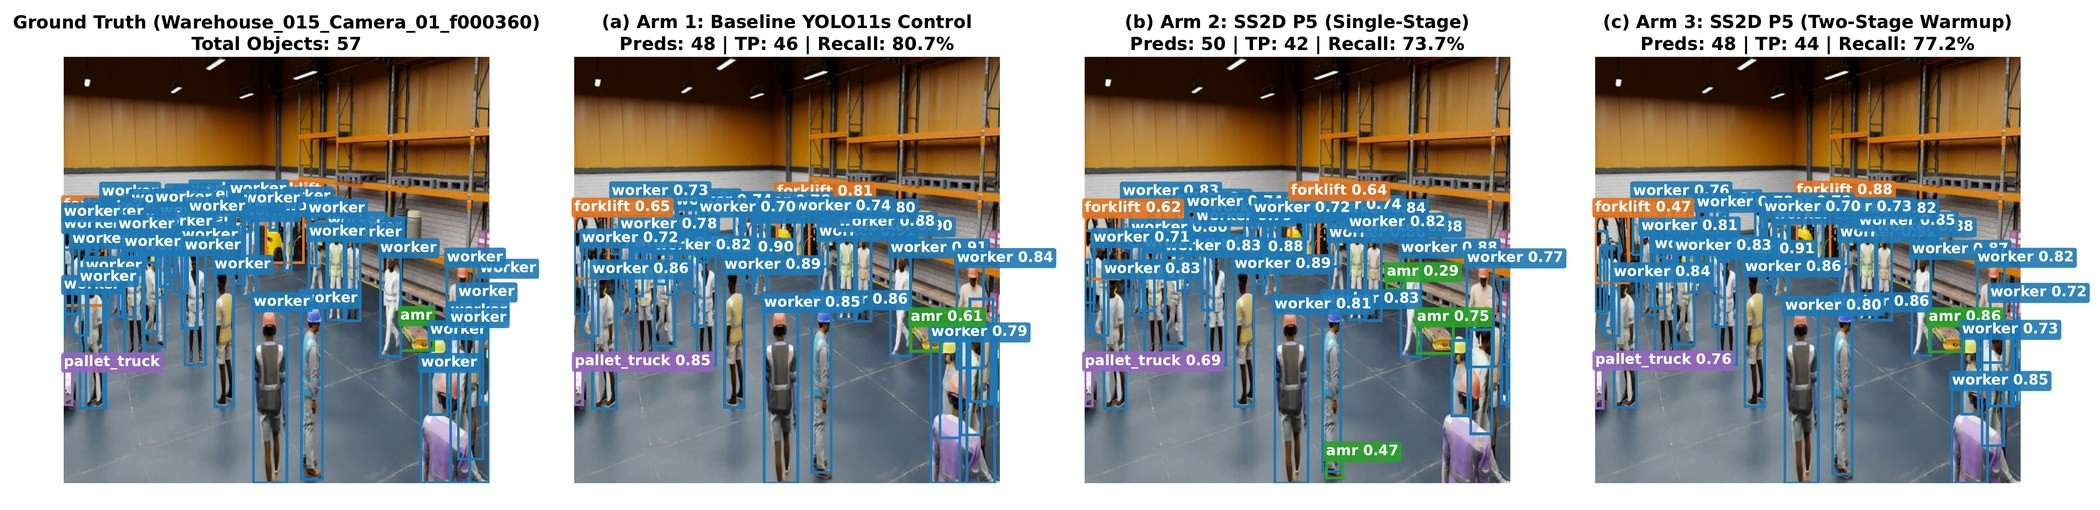
\includegraphics[width=\textwidth]{figures/fig_qualitative_f000360.jpg}
\caption{Predictions on validation frame \texttt{f000360} (\texttt{Warehouse\_015}, \texttt{Camera\_01}): ground truth, Arm~1, Arm~2, and Arm~3 (best-fitness checkpoints, confidence $\ge 0.25$, NMS IoU $0.45$), with the number of predictions, true positives (same class, $\text{IoU} \ge 0.5$, one match per ground-truth box), and recall.}
\label{fig:qualitative_comparison}
\end{figure}

\subsection{Edge Deployment}
\label{sec:res_edge}
Static savings do not carry over to deployment. Although SS2D-P5 has $0.63$\,M fewer parameters ($2.4$\,MiB in FP32), its ONNX file is larger ($38.5$ vs.\ $36.2$\,MiB) because the unrolled graph stores per-step constants (the same weights exported as a parallel scan take $34.7$\,MiB), and Table~\ref{tab:edge_runtime} shows that on the Cortex-A72 it is slower than the baseline by $5.7\%$ with one thread and $17.6\%$ with four threads. Its peak memory on the Pi is $373.6$\,MiB, $63.5\%$ below a $1$\,GiB budget but $60.1\%$ above the baseline ($233.4$\,MiB); SS2D-P4P5 peaks at $718.3$\,MiB. With four threads the Pi reaches $0.76$\,FPS for SS2D-P5, $0.52$\,FPS for SS2D-P4P5, and $0.90$\,FPS for the baseline, excluding preprocessing and NMS; the CPU results therefore establish operator portability and fit within $1$\,GiB, not real-time capability.

\begin{table}[t]
\caption{ONNX Runtime forward-pass latency and memory on the Raspberry Pi~4 ($640 \times 640$, batch size 1, FP32). Mem.: peak RSS. Rel.: median relative to the baseline of the same session and thread count.}
\label{tab:edge_runtime}
\centering
\footnotesize
\setlength{\tabcolsep}{3pt}
\begin{tabular}{llccccc}
\toprule
\textbf{Model} & \textbf{Threads} & \textbf{Mem.\ (MiB)} & \textbf{Median (ms)} & \textbf{Mean $\pm$ SD (ms)} & \textbf{Rel.} & \textbf{FPS} \\
\midrule
\multicolumn{7}{l}{\textit{Session~2 (100 calls with 1 thread, 30 with 4)}} \\
Baseline & 1 & 233.2 & 3192.88 & 3194.63 $\pm$ 5.0 & 1.00 & 0.31 \\
SS2D-P5 & 1 & 373.1 & 3374.10 & 3374.58 $\pm$ 3.6 & 1.06 & 0.30 \\
Baseline & 4 & 233.4 & 1117.27 & 1120.62 $\pm$ 7.5 & 1.00 & 0.90 \\
SS2D-P5 & 4 & 373.6 & 1314.26 & 1316.11 $\pm$ 4.8 & 1.18 & 0.76 \\
\midrule
\multicolumn{7}{l}{\textit{Session~1 (100 calls with 1 thread, 30 with 4)}} \\
Baseline & 1 & 233.2 & 3360.50 & 3360.15 $\pm$ 5.2 & 1.00 & 0.30 \\
SS2D-P4P5 & 1 & 716.5 & 4178.68 & 4178.96 $\pm$ 3.5 & 1.24 & 0.24 \\
Baseline & 4 & 233.3 & 1106.76 & 1110.09 $\pm$ 7.3 & 1.00 & 0.90 \\
SS2D-P4P5 & 4 & 718.3 & 1927.71 & 1929.04 $\pm$ 7.7 & 1.74 & 0.52 \\
\bottomrule
\multicolumn{7}{p{0.95\textwidth}}{\scriptsize Relative to session~2, the session-1 baseline median is $5.2\%$ higher with one thread (the clock of the session-1 single-thread runs was not logged) and $0.9\%$ lower with four threads.} \\
\end{tabular}
\end{table}

\textbf{Why the cheaper model is slower.} Table~\ref{tab:graph_profile} points to the scan's many small operators. (1)~Exporting the four-direction scan unrolls its loop over $L = 400$ steps into $14{,}771$ ONNX nodes ($4{,}800$ \texttt{Gather}, $3{,}293$ \texttt{Mul}, $3{,}212$ \texttt{Unsqueeze}, $1{,}621$ \texttt{Add}, $1{,}600$ \texttt{ReduceSum}), versus $320$ for the baseline; ONNX Runtime removes only $70$ of them. SS2D-P4P5 has $90{,}201$ nodes. (2)~Convolution time per call is nearly constant ($905$, $865$, and $877$\,ms), but its share of kernel time falls from $78.4\%$ to $50.0\%$ (SS2D-P5) and $22.5\%$ (SS2D-P4P5), while the scan's element-wise and indexing operators take $35.1\%$ and $68.4\%$. The profiler's per-node overhead (mean profiled call $1161$, $1951$, and $4943$\,ms) inflates these shares; the constant convolution time is more robust. With the small analytical cost of the scan (Section~\ref{sec:complexity}), this indicates that the extra latency comes from the operators executed per call rather than from arithmetic. (3)~Going from one to four threads speeds up the baseline by $2.86\times$ but SS2D-P5 by only $2.57\times$ (session~2), and the baseline by $3.04\times$ but SS2D-P4P5 by $2.17\times$ (session~1), consistent with a long chain of small dependent operators that leave little work to parallelize.

\begin{table}[t]
\caption{ONNX graph size and operator profile on the Pi (four threads, five profiled calls). Conv/scan: share of summed kernel time taken by convolutions and by the scan operators (\texttt{Mul}, \texttt{Squeeze}, \texttt{Unsqueeze}, \texttt{Add}, \texttt{ReduceSum}, \texttt{Gather}, \texttt{Split}).}
\label{tab:graph_profile}
\centering
\footnotesize
\setlength{\tabcolsep}{3.4pt}
\begin{tabular}{lccccc}
\toprule
\textbf{Model} & \textbf{Nodes} & \textbf{After ORT opt.} & \textbf{ONNX (MiB)} & \textbf{Conv (ms/call)} & \textbf{Conv / scan (\%)} \\
\midrule
Baseline & 320 & 236 & 36.2 & 905 & 78.4 / $<2.5$ \\
SS2D-P5 & 14{,}771 & 14{,}701 & 38.5 & 865 & 50.0 / 35.1 \\
SS2D-P4P5 & 90{,}201 & 72{,}385 & 46.6 & 877 & 22.5 / 68.4 \\
\bottomrule
\multicolumn{6}{p{0.92\textwidth}}{\scriptsize Baseline and SS2D-P4P5 profiled in session~1 without a clock log, SS2D-P5 in session~2 at $1.5$\,GHz.} \\
\end{tabular}
\end{table}

\textbf{Runtime intervention.} These observations are correlational, so we changed the graph form of the scan while keeping its computation fixed (Table~\ref{tab:g1_intervention}). First, removing the $P_5$ block entirely lowers latency by only $2.4\%$ (one thread) and $5.3\%$ (four threads), and the convolution-only block costs about the same, whereas the SS2D block adds $17.0\%$ and $22.2\%$ over the identity model. Second, fewer nodes did not mean lower latency: one ONNX \texttt{Loop} per direction shrinks the graph from $14{,}767$ to $367$ nodes but makes the model $2.2\times$ and $4.5\times$ slower than the unrolled scan, because its $37$--$38$-node body runs $400$ times per direction, about $60{,}000$ node executions per call. The chunked scan cuts the graph by $43\%$ but adds computation within each chunk and is $4.4\%$ and $14.0\%$ slower. Third, removing the dependency chain did not help either: a parallel associative scan~\cite{blelloch1990prefix} evaluates the same recurrence in $\lceil \log_2 L \rceil = 9$ whole-sequence steps with $619$ nodes (about $540$ after ONNX Runtime graph optimization, mostly \texttt{Mul}, \texttt{Slice}, \texttt{Pad}, and \texttt{Add}; no fused scan kernel), yet with the trained Arm~3 weights it is $20\%$ (one thread) and $64\%$ (four threads) slower than the unrolled export, and its one-to-four-thread speed-up drops to $1.81\times$ (baseline $2.73\times$, unrolled $2.48\times$). Fourth, removing arithmetic did not help: computing $\mathbf{W}_{\text{proj}}$ once removes $88.5$ of the $131.1$\,M MACs of the scan core, yet the export is $0.3\%$ (one thread) and $2.7\%$ (four threads) slower than the unrolled one. Neither node count, the sequential chain, nor the core's arithmetic is thus the cause on its own; the two forms pay different costs for the same small arithmetic ($13.1$\,M MACs). The unrolled scan executes a long chain of small dependent operators, whereas the parallel scan repeatedly reads and writes the full $400 \times 256 \times 16$ state of each direction ($6.25$\,MiB per tensor). Hardware counters (\texttt{perf stat}, one thread) support both: against the unrolled scan, the parallel scan retires $7\%$ more instructions but takes $25\%$ more cycles (IPC $0.76$ vs.\ $0.89$) with $2.2\times$ the estimated DRAM traffic, while the unrolled scan retires $10\%$ more instructions than the baseline at the same IPC. Fused kernels and the matrix (SSD) form of Mamba-2~\cite{dao2024mamba2}, which requires a scalar decay per head and thus a modified, retrained block, remain untested. The untrained upper block is not comparable with Table~\ref{tab:edge_runtime} in absolute terms (one-thread offset $6.5\%$). Only within-session ratios are interpreted (the session-4 baseline is up to $4.9\%$ off session~2); they reproduce the SS2D-P5 overhead of Table~\ref{tab:edge_runtime} ($1.06\times$ and $1.17\times$). Creating a session for the unrolled graph also takes $46$--$47$\,s (one or four threads), against $0.3$--$0.5$\,s for the baseline and the parallel scan.

\begin{table}[t]
\caption{Runtime intervention on the Pi: median latency in ms; Rel.: relative to the baseline of the same block at the same thread count; MiB: peak RSS with four threads. Upper block: session~2, untrained exports, 3 warmup and 20 timed calls (SD at most $10.8$\,ms). Lower block: session~4, trained Arm~1 and Arm~3 exports, protocol of Table~\ref{tab:edge_runtime} (SD at most $26.0$\,ms).}
\label{tab:g1_intervention}
\centering
\footnotesize
\setlength{\tabcolsep}{5pt}
\begin{tabular}{lcccccc}
\toprule
\textbf{Variant} & \textbf{Nodes} & \textbf{1 thread} & \textbf{Rel.} & \textbf{4 threads} & \textbf{Rel.} & \textbf{MiB} \\
\midrule
Baseline (\texttt{C2PSA}) & 320 & 3146.7 & 1.00 & 1132.8 & 1.00 & 233.3 \\
$P_5$ block removed & 292 & 3070.4 & 0.98 & 1072.7 & 0.95 & 229.4 \\
Convolution-only & 300 & 3105.4 & 0.99 & 1095.9 & 0.97 & 230.5 \\
SS2D, unrolled & 14{,}767 & 3593.8 & 1.14 & 1311.3 & 1.16 & 373.6 \\
SS2D, ONNX \texttt{Loop} & 367 & 7778.6 & 2.47 & 5938.4 & 5.24 & 274.0 \\
SS2D, chunked ($T = 4$) & 8{,}355 & 3752.5 & 1.19 & 1494.7 & 1.32 & 304.3 \\
\midrule
\multicolumn{7}{l}{\textit{Trained exports, session~4}} \\
Baseline (\texttt{C2PSA}) & 320 & 3204.1 & 1.00 & 1171.8 & 1.00 & 233.4 \\
SS2D, unrolled & 14{,}771 & 3396.6 & 1.06 & 1370.8 & 1.17 & 373.6 \\
SS2D, $\mathbf{W}_{\text{proj}}$ once & 14{,}773 & 3407.0 & 1.06 & 1407.4 & 1.20 & 374.1 \\
SS2D, parallel scan & 619 & 4089.6 & 1.28 & 2253.6 & 1.92 & 389.6 \\
\bottomrule
\multicolumn{7}{p{0.92\textwidth}}{\scriptsize Session creation with four threads: $0.26$\,s (baseline), $47.3$\,s (unrolled), $44.7$\,s ($\mathbf{W}_{\text{proj}}$ once), $0.34$\,s (parallel scan).} \\
\end{tabular}
\end{table}

\subsection{Design Lessons and Limitations}
\label{sec:limitations}
Three lessons follow for replacing attention with selective scans in small detectors. (1)~\emph{Fewer FLOPs can mean a slower model}, and neither a smaller graph, a parallel scan, nor less arithmetic necessarily helps on a CPU; latency and memory should be measured at the deployed thread count. (2)~\emph{Comparisons need identical warm starts}: the class-agnostic box-regression branch must be transferred for every arm. In a two-epoch pilot with an earlier version of the block, in which this branch was not transferred, the SS2D model reached $0.09\%$ $\text{mAP}_{50}$ against $39.8\%$ for the baseline (training box loss $4.50$ vs.\ $1.30$); all reported arms transfer it. (3)~\emph{A zero-initialized convolution ahead of BN is not an identity initialization}; zero-$\gamma$ initialization (Eq.~\eqref{eq:zero_gamma}) avoids the problem by construction, although its effect on detector training remains to be measured.

The results have clear limitations. All accuracy results come from one seed, a 20-epoch budget, and one $100$-frame validation facility that also served for checkpoint selection, without a held-out test facility or significance testing. The data are synthetic, cover two facilities, and consecutive frames are highly correlated. The reported SS2D models use the initialization of Eq.~\eqref{eq:zero_wout}, and because Arm~3 combines freezing with a restarted schedule, its differences from Arm~2 cannot be attributed to either factor alone. Identity and convolution-only replacements were measured for runtime only, so no trained ablation separates the scan from the removal of \texttt{C2PSA}, and the simplifications relative to Mamba are not ablated. Edge measurements cover only the forward pass on one embedded CPU in FP32; preprocessing, NMS, the session creation of SS2D-P4P5 (tens of minutes, not timed), accelerators, quantization, and energy were not measured. The Pi results come from five sessions, and most intervention variants use untrained exports.

\section{Conclusion}
\label{sec:conclusion}
\textbf{RQ1.} Replacing \texttt{C2PSA} with a plugin-free 2D selective scan removes $63.9\%$ of the Layer-10 parameters and $6.72\%$ of the model at $21.2$ instead of $21.7$ GFLOPs, but does not preserve overall accuracy in our single-seed experiments: all SS2D variants have lower $\text{mAP}_{50-95}$, and the baseline has the highest final-epoch $\text{mAP}_{50}$. The higher forklift accuracy of the SS2D variants ($75.3$--$79.7\%$ vs.\ $70.1\%$) coincides with forklifts being the largest objects, but remains to be confirmed across seeds and attributed with trained ablations. \textbf{RQ2.} Two-stage training gave mixed results (higher final-epoch but lower best-fitness accuracy than single-stage training, with a shifted operating point). The zero-initialized output convolution preserves identity only at step $0$; we therefore cannot conclude whether a dedicated protocol is necessary. \textbf{RQ3.} The model runs on a Raspberry Pi~4 without plugins and within $1$\,GiB ($373.6$\,MiB), but it is slower than the baseline ($1314$ vs.\ $1117$\,ms with four threads, $+18\%$; $+6\%$ with one thread). The overhead follows how the scan is executed, not its arithmetic or graph size: an ONNX \texttt{Loop} with $367$ nodes, a chunked scan, and a parallel associative scan with $619$ nodes and no sequential chain were all slower than the unrolled scan with $14{,}767$--$14{,}771$ nodes (the parallel scan by $64\%$ with four threads), computing the shared projection once ($-68\%$ of the core's MACs) did not lower latency, and removing \texttt{C2PSA} altogether saved only $2$--$5\%$.

Future work will re-train all arms with zero-$\gamma$ and Mamba-style step-size initialization over multiple seeds, with trained identity and convolution-only ablations and a held-out test facility; measure fused scan kernels and an SSD-style block with scalar decays, also on accelerators and with quantization; and evaluate on real warehouse footage.

\begin{credits}
\subsubsection{\ackname} \ifanonymous Funding information anonymized for review.\else This research is funded by Ho Chi Minh City Open University.\fi{} We thank the Ultralytics and PhysicalAI-SmartSpaces developers for releasing their code and data.

\subsubsection{\discintname} The authors have no competing interests to declare that are relevant to the content of this article.
% The repository must be public before submission if it is cited here.
\subsubsection{Code Availability.} \ifanonymous Code, weights, ONNX exports, and logs are in the supplementary material.\else Code, logs, checkpoints, and ONNX models: \url{https://github.com/h4nsx/nckh}.\fi
\end{credits}


\bibliographystyle{splncs04}
\bibliography{references}

\end{document}
